%% ------------------------------------------------------------------------- %%
\chapter{Arquitetura proposta}
\label{cap:modelo}
    
Como visto no capítulo \ref{cap:aspectos-basicos}, a proposição de uma arquitetura visando à integração de dados na Internet não é um processo trivial e demanda o conhecimento em diferentes áreas de pesquisa tais como a Web Semântica e a Integração de Dados.

Um dos principais pontos para a integração da informação na Internet é a definição de uma estrutura que represente com clareza um determinado domínio de conhecimento, como  explicado por \citet{May} e \citet{Ahmed2008}. Além disso é preciso estabelecer mecanismos capazes de interpretar e identificar os dados relevantes sobre os documentos de dados expostos na Web e convertê-los sobre a semântica comum estabelecida anteriormente. É preciso também considerar o acesso à informação pois, uma vez que os dados estão centralizados, eles podem (e serão) consultados por diferentes usuários interessados na informação ali contida. Nesse contexto, uma arquitetura capaz de promover a interoperabilidade de informações na Internet deve conter ao menos uma camada de recuperação de dados, uma camada de persistência e centralização da informação e uma camada de apresentação para o acesso à informação, conforme ilustrado pela Figura~\ref{fig:arquitetura_integracao_dados}.

\begin{figure}[!ht]
  \centering
  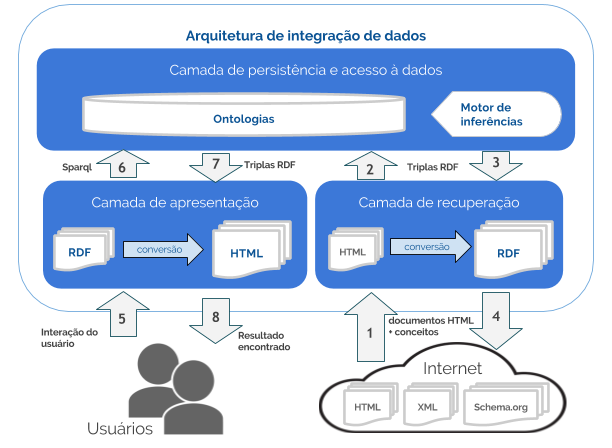
\includegraphics[width=.90\textwidth]{arquitetura_integracao_dados} 
  \caption{Proposta de arquitetura de sistema de integração de dados da Web}
  \label{fig:arquitetura_integracao_dados} 
\end{figure}

Cada uma destas camadas, bem como os diversos processo envolvidos, são descritos a seguir.

\section{Escolha do domínio de dados}
\label{sec:camada_de_recuperacao_de_dados}

Do ponto de vista pragmático, uma primeira decisão a ser tomada num projeto do tipo proposto neste trabalho é delimitar o escopo de dados em um domínio previamente estabelecido. Além disto, devem-se determinar as as fontes de dados que serão utilizadas.

Neste trabalho os domínios de informação escolhidos são eventos e restaurantes. São vários os portais que divulgam exposições, peças de teatros, palestras, aulas, entre outros. No entanto, uma informação sobre um determinado evento está distribuída nessas diferentes fontes de dados, o que dificulta uma visão centralizada sobre os eventos que acontecem em determinada data, horário ou região. Nesse contexto, a existência de um sistema capaz de responder esses questionamentos de maneira centralizada pode ser importante para alcançar uma visão mais ampla e auxiliar a tomada de decisão do usuário final. Neste trabalho, espera-se responder a um usuário, de maneira centralizada, os eventos de uma determinado região, os eventos que acontecem em um determinado dia e os eventos de um determinado tipo como, por exemplo, os diferentes eventos que acontecem perto e uma determinada referência de geolocalização. 

Quanto às fontes de dados utilizadas, neste trabalho adotam-se  os portais Guia Da Semana\footnote{\url{https://www.guiadasemana.com.br/}}, Guia da Folha\footnote{\url{http://guia.folha.uol.com.br/}} e o portal de Eventos da USP\footnote{\url{http://www.eventos.usp.br/}} conforme apresentado na Figura~\ref{fig:fontes_de_dados}. Os dois primeiros portais foram escolhidos em razão de serem amplamente conhecidos e utilizados, além de possuírem uma ampla base de dados sobre eventos e restaurantes. Já o portal da USP foi escolhido por manter uma grande quantidade de eventos acadêmicos dentro do contexto da Universidade de São Paulo. 

\begin{figure}[!ht]
  \centering
  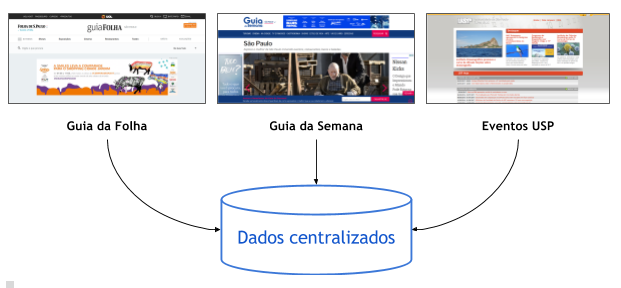
\includegraphics[width=.85\textwidth]{fontes_de_dados} 
  \caption{Fontes de dados sobre eventos e restaurantes}
  \label{fig:fontes_de_dados} 
\end{figure}

\section{Definição de uma ontologia}
\label{sec:ontologia}

A fim de integrar fontes provenientes de diferentes portais de eventos dos quais não temos domínio sobre o conteúdo exposto, é necessário adotar uma estrutura comum previamente definida.i.e. uma ontologia, bem como construir um modelo de conversão de dados de cada uma destas fontes para esta estrutura comum. Neste trabalho, o processo de extração, transformação e persistência dos dados é ilustrado na Figura~\ref{fig:extracao_de_dados}. Em primeiro lugar, os dados são recuperados dos portais de eventos escolhidos a partir de técnicas de recuperação de informação usando expressões regulares. O conteúdo selecionado é então mesclado com uma ontologia, gerando assim uma informação semanticamente anotada. Por fim, a informação é então armazenada em um repositório de dados para acesso baseado em ontologias. Como resultado deste processo, obtém-se um repositório de dados semanticamente anotado que pode ser consultado de maneira centralizada. 

Conforme já relatado na seção~\ref{sec:schema_org} do Capitulo~\ref{cap:aspectos-basicos}, o portal Schema.org \citep{Mika2015} apresenta definições de conceitos padronizadas e amplamente revisados, inclusive por esforços de iniciativa privada como no caso de Google e Microsoft.
    
\begin{figure}[!ht]
  \centering
  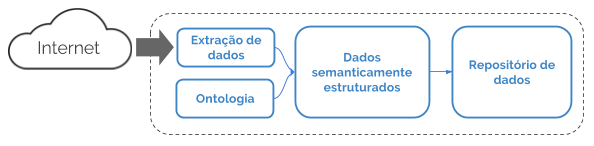
\includegraphics[width=.85\textwidth]{extracao_de_dados} 
  \caption{Processo de extração e persistência de dados}
  \label{fig:extracao_de_dados} 
\end{figure}

Neste trabalho serão utilizados os conceitos ``Estabelecimento de alimentos'' (FoodEstablishment), ``Evento'' (Event) e suas respectivas derivações,  como apresentado na hierarquia de conceitos da Figura~\ref{fig:hierarquia_de_conceitos}. Nesta figura,   todas os conceitos são derivados do conceito abstrato  ``Thing''. Definem-se conceitos tais como  exposições (``ExhibitionEvent''), sessões de cinema (``ScrenningEvent''), e peças de teatro (``TheaterEvent''), entre outros.  Herda-se também as declarações de propriedades para cada classificação, i.e, o título, latitude, longitude, descrição, data e horário do evento, além de especificações mais restritas aos níveis mais inferiores da hierarquia;  por exemplo, o tipo de comida, que só será válido para ``Restaurant'', para classificar se o restaurante oferece comida italiana, mexicana ou japonesa.

\begin{figure}[!ht]
  \centering
  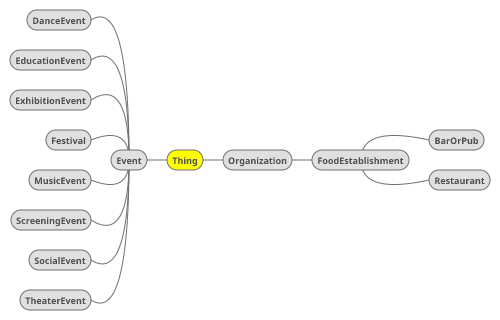
\includegraphics[width=.85\textwidth]{hierarquia_de_conceitos} 
  \caption{Hierarquia de conceitos}
  \label{fig:hierarquia_de_conceitos} 
\end{figure}

\section{Preparação e recuperação de dados}
\label{sec:preparacao_recuperacao_dados}

Uma vez definido  o domínio de dados, as fontes de informação e as ontologias,  deve-se então  identificar e extrair a informação relevante nos portais escolhidos. Na proposta deste trabalho, a camada de recuperação de dados contém toda a inteligência para a extração de informação relevante nos portais selecionados. Em outras palavras, é o módulo responsável pela mediação da requisição para uma fonte de dados na Internet e a consequente transformação daquele conteúdo escolhido para um documento RDF válido conforme representado pelas setas 1 e 4 na Figura~\ref{fig:arquitetura_integracao_dados}. Para tal, é necessário criar  um conjunto de regras baseadas em expressões regulares específicas a cada fonte de dados escolhida, transformando assim em tempo real as informações relevantes em dados semanticamente anotados a partir de triplas RDF coerentes que podem ser entendidas por máquinas.

O reconhecimento do conteúdo significativo nos diferentes portais não é uma tarefa trivial. Para cada fonte de dados, é necessário analisar e identificar os padrões de repetição de dados apresentados dentro de cada domínio de interesse. Embora cada portal da Web utilize em comum o protocolo  HTML para expor a informação que é dinamicamente produzida, a estrutura desses documentos é geralmente muito diferente. Tal característica é esperada, uma vez que são diferentes profissionais construindo modelos de apresentação específicos distanciando-se assim de padronizações. Desse modo, o mapeamento entre onde estará um determinado conteúdo não será o mesmo para dois portais distintos; por outro lado, uma vez identificado um padrão para uma fonte de dados, este pode ser reaproveitado para todas as outras páginas do mesmo portal. 

\begin{figure}[!htb]
  \centering
  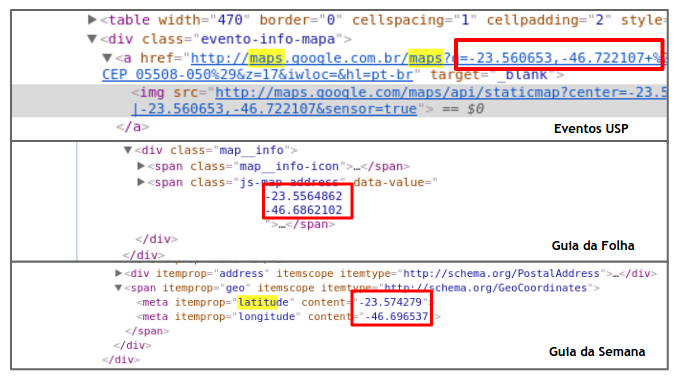
\includegraphics[width=.85\textwidth]{identificacao_de_padroes_html_2} 
  \caption{Extração de latitude e longitude em diferentes portais}
  \label{fig:identificacao_de_padroes_html} 
\end{figure}

Os exemplo contidos nas Figuras~\ref{fig:identificacao_de_padroes_html} e~\ref{fig:repeticao_padroes_html} ilustram com maior clareza essa condição. Neles é possível observar que a apresentação do conteúdo nessas páginas é diferente e isso ocorre não só por causa dos dados ali publicados, mas também porque a estrutura do documento que é interpretado pelo navegador difere em cada portal. Tomando como exemplo a Figura~\ref{fig:identificacao_de_padroes_html} vemos que a captura dos dados de latitude e longitude é diferente para cada portal. Apesar disso, esse padrão se repete para todo conteúdo específico daquele portal, como é possível notar através da Figura~\ref{fig:repeticao_padroes_html}. Nesse exemplo a captura do título de um evento sempre está delimitada por marcações especificas no documento HTML (<h1>). Sendo assim, embora seja uma tarefa simples para os humanos identificar e interpretar a informação de coordenadas geográficas da latitude e longitude dos exemplos propostos, isto não ocorre para um processamento automático.

\begin{figure}[!htb]
  \centering
  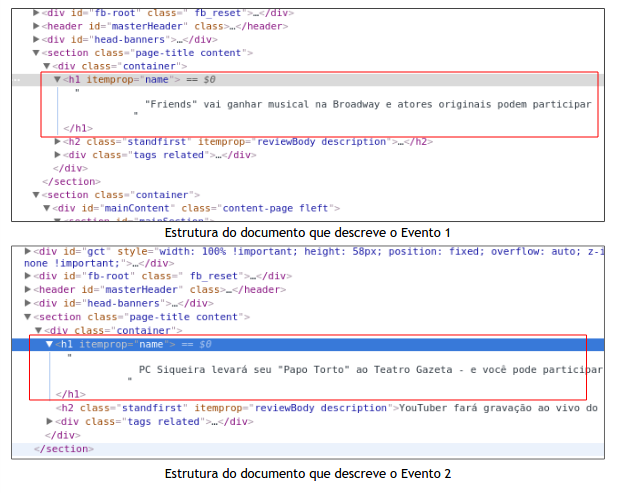
\includegraphics[width=.85\textwidth]{repeticao_padroes_html} 
  \caption{Repetição de padrão no portal Guia da Semana}
  \label{fig:repeticao_padroes_html} 
\end{figure}

Neste trabalho, foram elaborados mecanismos com capacidade de interpretar e transformar o conteúdo de cada um dos portais escolhidos em informações com semântica agregada. O primeiro passo para a sua construção é a análise da estrutura do documento HTML produzido dinamicamente por cada um dos portais escolhidos escolhidos quando um determinado conteúdo é acessado. A partir desse conhecimento, torna-se possível entender onde e como que a informação se repete na estrutura sintática do objeto produzido. Essa observação é então transcrita por meio de diferentes expressões regulares que mapeiam cada propriedade identificada no documento para um conceito do portal Schema.org. 

A Figura~\ref{fig:repeticao_padroes_endereco_guia_semana} exemplifica o processo de identificação e extração do endereço de um evento no portal Guia da Semana a partir do uso de expressões regulares. Desse modo, a partir da junção de diferentes expressões regulares trabalhando conjuntamente sobre o conteúdo dos diferentes documentos dos portais escolhidos é que emerge a inteligência da interpretação do conteúdo relevante nesses portais. Finalmente, toda a informação recuperada é então transformada em triplas RDF que podem ser armazenadas em uma base de dados para consultas posteriores.

\begin{figure}[!hbt]
  \centering
  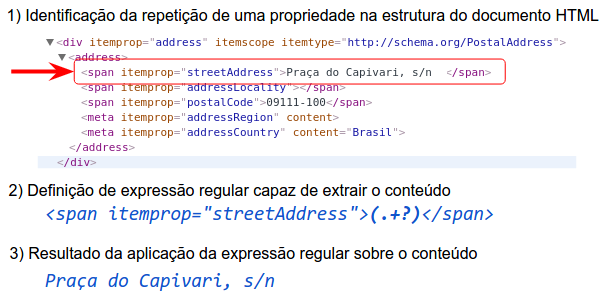
\includegraphics[width=.85\textwidth]{repeticao_padroes_endereco_guia_semana} 
  \caption{Processo de extração de um endereço no portal Guia da Semana}
  \label{fig:repeticao_padroes_endereco_guia_semana} 
\end{figure}

\section{Persistência e centralização de dados}
\label{sec:persistencia_e_centralizacao_de_dados}

A camada de persistência e centralização de dados é o coração da arquitetura proposta neste trabalho. É sua  a responsabilidade de armazenar todas as informações que foram recuperadas a partir dos portais escolhidos, resolver conflitos de informação, permitir a inferência de dados e disponibilizar mecanismos para recuperação da informação. Conforme ilustra a Figura~\ref{fig:centralizacao_dados}, todas as triplas RDF criadas são incluídas em uma base de dados centralizada para que o acesso aos dados baseado em ontologias possa ser realizado. Esse processo é representado na arquitetura do sistema (Figura~\ref{fig:arquitetura_integracao_dados}) pela seta 2, que representa a persistência das triplas RDF, e pela seta 3 que representa os processos decorrentes da transformação de documentos expostos na Web para triplas RDF. Além disso, é atribuição deste módulo centralizar os dados e resolver possíveis conflitos entre informações extraídas.

\begin{figure}[!ht]
  \centering
  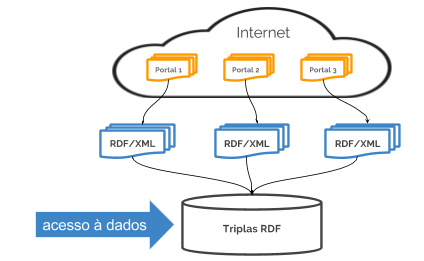
\includegraphics[width=.85\textwidth]{centralizacao_dados} 
  \caption{Centralização e ponto de acesso a dados}
  \label{fig:centralizacao_dados} 
\end{figure}

A recuperação dos dados em um único ponto centralizado é uma característica interessante no contexto da Internet. Dada a natureza descentralizada da rede, na qual a informação está armazenada em diferentes servidores distribuídos na Web, um mecanismo de consultas e inferência sobre toda essa informação deve levar em consideração essa característica. Entre os diferentes problemas que a pesquisa da informação na rede enfrenta está a velocidade de transferência de dados; esta é mais afetada quanto mais distante estão dois pontos alvos da recuperação da informação. Há também o caráter técnico que envolve a própria estrutura da Internet que não garante que um determinado servidor de informações estará acessível em um dado momento, seja por problemas da própria rede ou outros quaisquer. Além disso, ainda há o processo de inferência que demanda a recuperação de todo o conteúdo das diferentes as bases de dados de todas as organizações escolhidas. Esta opção se justifica pois  uma simples busca feita por um usuário em um modelo descentralizado pode não ser atendida em tempo hábil, uma vez que toda a informação contida nos diferentes portais escolhidos precisará ser obtida, armazenada e inferida a cada consulta. Neste trabalho, foi utilizado portanto um modelo centralizado de dados.

O modelo centralizado proposto neste trabalho se baseia em um banco de dados único construído a partir das informações obtidas diretamente das fontes de informações pré-estabelecidas. Ele é o resultado de um processo constante, realizado diariamente, da aplicação dos mecanismos de interpretação e recuperação discutidos anteriormente. Desse modo as informações sobre os eventos e restaurantes são adicionadas ou atualizadas de forma continua dentro do banco de dados semântico o que garante que alterações no conteúdo exposto pelos portais escolhidos sejam refletidas no banco de dados centralizado.

O acesso aos dados persistidos é outro fator importante e está representado pelas setas 6 e 7 da proposta de arquitetura ilustrada na Figura~\ref{fig:arquitetura_integracao_dados}. Para alcançar essa capacidade, a arquitetura proposta neste trabalho disponibiliza serviços para consultas SPARQL que são feitas diretamente sobre a base de informações elaborada e possibilitam consultas baseadas em ontologias. Além disso, também há serviços que executam a inferência sobre os dados contidos na base de dados. Desse modo, a inferência sobre os dados existentes pode ser realizada a qualquer momento.

\section{Resolução de duplicações e conflitos}
\label{sec:resolucao_de_conflitos}

A resolução de duplicações e conflitos é um fator importante no que diz respeito à centralização de dados. Tomando como base o contexto de publicadores de eventos na Internet, embora o conteúdo existente em cada um desses portais seja geralmente complementar, isso é, cada site focado em uma região ou tipo de informação especifica, pode ocorrer que a mesma informação esteja duplicada em diferentes portais ao mesmo tempo, conforme ilustra o exemplo da Figura~\ref{fig:mesmo_evento_diferentes_portais}. Na figura, a informação sobre a peça de teatro ``Lés Misérables'' aparece ao mesmo tempo em portais distintos.

\begin{figure}[!ht]
  \centering
  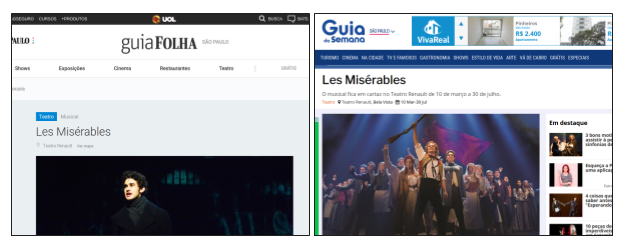
\includegraphics[width=.85\textwidth]{mesmo_evento_diferentes_portais} 
  \caption{Conflito de informações em diferentes portais}
  \label{fig:mesmo_evento_diferentes_portais} 
\end{figure}

Há diferentes formas para a identificação de dados similares. No entanto, a escolha de uma forma em detrimento de outra pode ser pautada pelo tipo de dado que está sendo tratado. No caso dos eventos e restaurantes tratados neste trabalho, o título de uma peça de teatro, o nome de um filme no cinema, o nome de um restaurante e até mesmo o título de uma exposição é sempre fixo, mesmo que exposto em diferentes portais. Exemplo disso é a peça ``Les Misérables'', que é discriminada da mesma maneira nos diferentes portais em que esta publicada. Essa característica dos eventos foi explorada neste trabalho para identificar que se trata do mesmo evento.

Além de duplicações, pode ocorrer conflito de informação, quando duas fontes distintas fornecem informações diferentes sobre um mesmo evento. No domínio tratado neste trabalho, um exemplo de tal conflito poderia ser o fato de dois portais fornecerem informações distintas a respeito do horário de início do mesmo evento. 

Além das responsabilidades de centralizar a informação, realizar inferências e expor um ponto de acesso aos dados, a camada de persistência ainda dispõe de inteligência para a resolução de conflitos. Essa característica é definida a partir de um módulo especializado capaz de decidir, a partir de comparações simples, se um determinado dado deve prevalecer sobre outro semelhante, evitando assim a inconsistência da informação. Nele, o processo de decisão emerge a partir de uma seqüência de regras bem definidas. 

A resolução de conflitos neste trabalho se dá através de um processo de avaliação baseado em regras pré-definidas, criadas a partir do domínio dos dados escolhido, conforme ilustrado na Figura~\ref{fig:hierarquia_resolucao_conflito}. O primeiro passo da resolução de conflitos é a comparação das informações, através de valores da tripla RDF no qual uma consulta SPARQL é realizada diretamente na base de dados, utilizando como parâmetros de filtragem os dados do sujeito e do predicado da tripla RDF. Quando a consulta não retorna um resultado,  a informação pode ser incluída na base de dados, já que se trata de uma nova informação; entretanto, quando dados são retornados, inicia-se uma segunda fase de validações.

\begin{figure}[!ht]
  \centering
  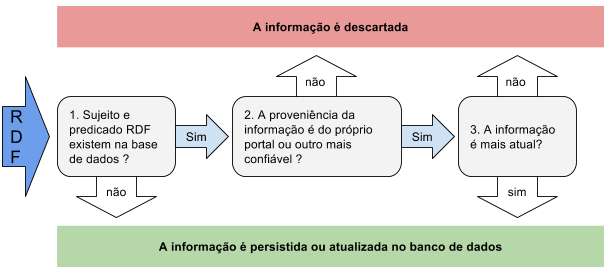
\includegraphics[width=.85\textwidth]{hierarquia_resolucao_conflito} 
  \caption{Processo de resolução de conflitos}
  \label{fig:hierarquia_resolucao_conflito} 
\end{figure}

A segunda fase de validação envolve a proveniência da informação. Isso significa que alguns dados são escolhidos em detrimento de outros, baseado em uma ordem de confiabilidade das fontes de informação. Desse modo, a decisão entre duas informações contidas em triplas que possuem objetos diferentes sendo uma extraída de um site A e de outro site B dependem da ordem de precedência pré-estabelecida. Supondo que se estabeleça que a informação do portal B é mais relevante que a do portal A pelo pelo fato deste último ter conteúdo mais preciso, possui menor desvio gramatical, maior abrangência territorial ou qualquer outro, então a informação de A será sempre substituída pela informação de B. Por fim, se a informação veio do próprio site e portanto não há ordem de preferência da informação, então os dados são substituídos e tratados como uma atualização da informação.

A fim de ilustrar o processo de resolução de conflitos, vamos tomar como base a peça ``A Era do Rock'' que existe tanto no portal Guia da Semana quanto no portal Guia da Folha. Neste trabalho, as informações provenientes do portal Guia da Folha foram definidas como prioritárias em relação às informações do Guia da Semana em virtude da abrangência de informação e da quantidade de revisores desse portal, que é maior que a do segundo. O primeiro passo é recuperar as informações do portal com prioridade menor, nesse caso o Guia da Semana. Como as triplas RDF geradas a partir da analise do conteúdo desse evento ainda não estão registradas, toda a informação descoberta é prontamente adicionada no banco de dados. A partir desse momento, a informação passa a ser extraída do portal Guia da Folha. Todas as propriedades que não forem encontradas no banco de dados são prontamente adicionadas na base de dados. Esse processo determina a mesclagem da informação dos diferentes portais sobre o mesmo evento. Por outro lado, as propriedades que já existem tais como título, data ou endereço, são prontamente atualizadas já que o portal Guia da Folha tem prioridade em relação ao Guia da Semana. 

Como a informação na Internet pode sofrer alterações, há um processo de atualização que realiza novamente a recuperação dos dados dentro de um período pré-definido. Levando em consideração o exemplo anterior, quando a informação é novamente recuperada do portal Guia da Semana, caso uma nova propriedade que ainda não exista no banco de dados seja detectada, ela será prontamente adicionada. Se a propriedade já existe, então a informação extraída do portal será descartada uma vez que sua prioridade de persistência é menor. Por outro lado, quando a informação é recuperada do portal Guia da Folha e caso a propriedade não exista, ela é prontamente adicionada; quando ela já existe, ela é atualizada. O ciclo de recuperação de informação é então mantido por tempo pré-definido. 

A geolocalização é um caso especial do processo de substituição de dados. Diferentemente das outras propriedades do conceito, a geolocalização não pode simplesmente substituir um valor pré-existente de um Restaurante, por exemplo. Um exemplo típico são franquias, onde a informação de latitude e longitude de um estabelecimento  especifico não pode simplesmente sobrescrever os dados pré-existentes.  Nesses casos, a informação sobre a latitude e longitude só é atualizada caso se encontre num raio de 5m da posição original. Caso contrário, uma nova informação é adicionada na base de dados.

\section{Regras para inferências sobre dados}
\label{sec:regras_inferencia_dados}

A proposta deste trabalho busca realizar a integração de dados disponibilizados na Internet a partir da centralização do conteúdo exposto em diferentes portais da Internet, adicionando uma camada semântica que permite realizar a busca de dados mais ricos no contexto de eventos culturais que acontecem na cidade de São Paulo. Nesse cenário, saber se um determinado lugar, como por exemplo um teatro ou uma exposição, é próximo a outro como um restaurante ou um pub pode ser interessante para que o usuário final possa programar sua agenda de acordo com a proximidade entre esses dois pontos. Uma das formas de se alcançar esse conhecimento é verificar se dois pontos são suficientemente próximos. Essa forma é custosa, pois exige um grande esforço manual por parte do indivíduo interessado nessa consulta. Outra forma mais eficiente é a definição de um conceito que explique o que é estar ``próximo'' e depois, por inferência sobre os dados, alcançar esse objetivo a partir de uma consulta baseada nesse significado. O conceito ``perto'' foi definido neste trabalho para atingir tal finalidade.

A regra ``perto de um lugar'' possibilita a busca de pontos de geolocalização que estão próximos. Essa condição é calculada a partir dos resultados de uma função que delimita a área na qual os estabelecimentos devem estar para serem considerados próximos e é ilustrada pela Figura~\ref{fig:regra_rdf_near}. No entanto, para que funcione corretamente, é preciso definir qual é a distância que deve ser considerada para poder inferir que dois locais estão localizados perto um do outro.  Neste trabalho, a distância de quinhentos metros foi escolhida por tratar-se de um espaço curto que pode ser percorrido em poucos minutos. Assim, caso  dois pontos ``a'' e ``b'' que possuem respectivamente as latitudes e longitudes (x1,y1) e  (x2,y2) estiverem distantes  em um raio de até quinhentos metros, então uma nova tripla ``?a iweb:near ?b'' é adicionada na base de dados sugerindo que ``a'' está perto de ``b''. A segunda regra da figura implementa o aspecto transitivo desta relação.

\begin{figure}[!ht]
    \begin{lstlisting}[language=XML]
@prefix schema: <http://schema.org/> .
@prefix iWeb: <http://integraWeb.ddns.net/> .

[rule1: (?a schema:latitude ?y1), (?a schema:longitude ?x1), (?b schema:latitude ?y2), (?b schema:longitude ?x2), near(?x1, ?y1, ?x2, ?y2) -> (?a iweb:near ?b)]
[rule2: (?a iweb:near ?b)-> (?b iweb:near ?a)]
    \end{lstlisting}
    \caption{Regra que define o conceito perto (near)}
    \label{fig:regra_rdf_near} 
\end{figure}

\section{Camada de apresentação}
\label{sec:camada_de_apresentacao}

A última camada da arquitetura proposta neste trabalho é a camada de apresentação. É nesta camada que se espera a interação entre o usuário e a fonte dos dados integrados a partir de uma página Web. Assim, a partir de consultas SPARQL, o usuário consegue obter os dados de interesse de forma centralizada, sem a necessidade deconsultar cada uma dos outros portais. Essa condição está representada pelas setas 5 e 8 na Figura~\ref{fig:arquitetura_integracao_dados}, que representam um usuário interagindo com um sistema que implementa a arquitetura apresentada neste trabalho.

A camada de apresentação simplifica a interação do usuário leigo com o sistema, ao gerar consultas utilizando a linguagem SPARQL de maneira transparente sem a necessidade de conhecimento prévio na linguagem. Essa condição se dá através de campos de pesquisa pré-definidos como, por exemplo, o tipo do evento ou do estabelecimento de interesse do usuário. No entanto, o sistema não se limita a essas condições e possibilita ao usuário mais avançado realizar uma consulta SPARQL diretamente no sistema, permitindo assim pesquisas mais elaboradas sobre o banco de dados. 

O resultado da consulta é desenhado em cima de uma mapa, que contém informações sobre ruas e estabelecimentos na região dos eventos e estabelecimentos encontrados. Um exemplo de tal saída é apresentado na Figura~\ref{fig:arquitetura_apresentacao}.

\begin{figure}[!ht]
  \centering
  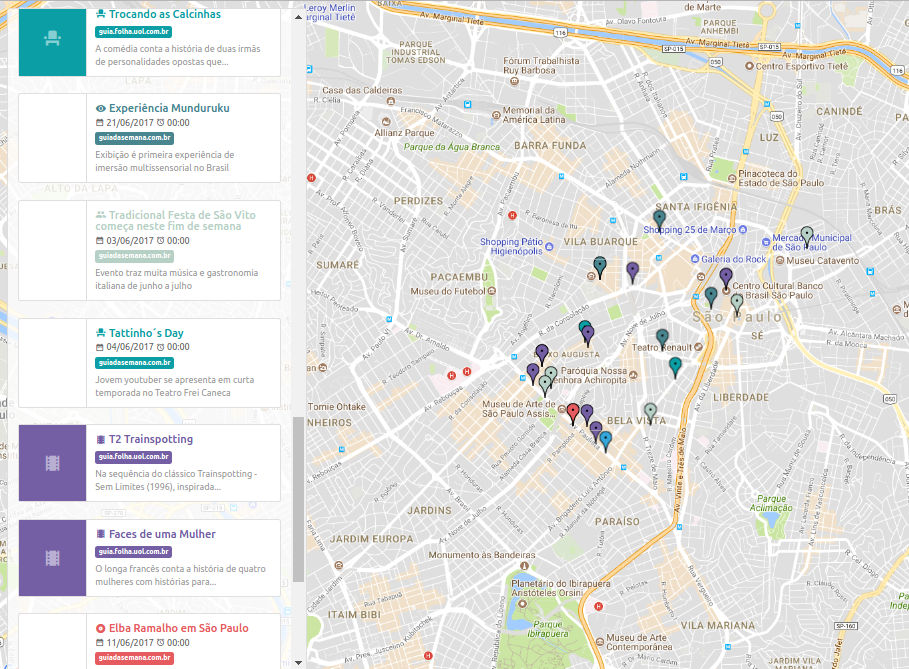
\includegraphics[width=.85\textwidth]{apresentacao_sistema} 
  \caption{Exemplo de apresentação de resultado de consulta}
  \label{fig:arquitetura_apresentacao} 
\end{figure}

Tal interface facilita a interação do usuário, pois atualmente são muitos os sistemas baseados em ferramentas que se valem de mapas, como o aplicativo Google Maps\footnote{\url{http://maps.google.com/}}, Uber, TripAdvisor, entre outros. Além disso, tal modo se apresentação auxilia no entendimento da informação do evento e sua distância em relação a outros pontos de referência identificados pelo usuário no próprio mapa. 

%\begin{figure}[!ht]
%  \centering
%  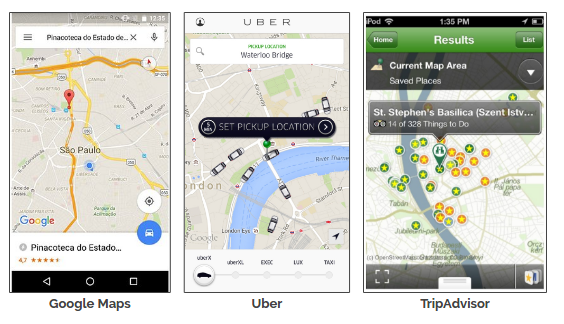
\includegraphics[width=.85\textwidth]{aplicativos_baseados_em_mapas} 
%  \caption{Interação com usuário baseada em mapas}
% \label{fig:aplicativos_baseados_em_mapas} 
%\end{figure}

No capítulo a seguir, apresentam-se os experimentos realizados com esta arquitetura.